\usetikzlibrary{calc}

\begin{frame}
\frametitle{2019ish measurement data}
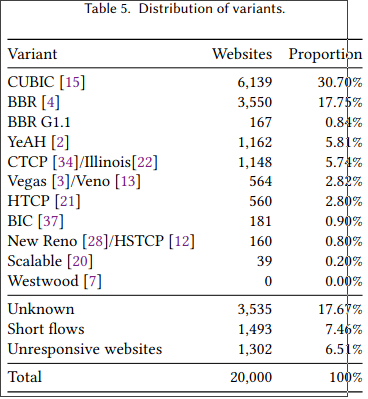
\includegraphics[height=0.9\textheight]{../congest/mishra-et-al-table5}
\imagecredit{Mishra et al, ``The Great Internet TCP Congestion Control Census''}
\end{frame}

\begin{frame}
\frametitle{2023ish measurement data}
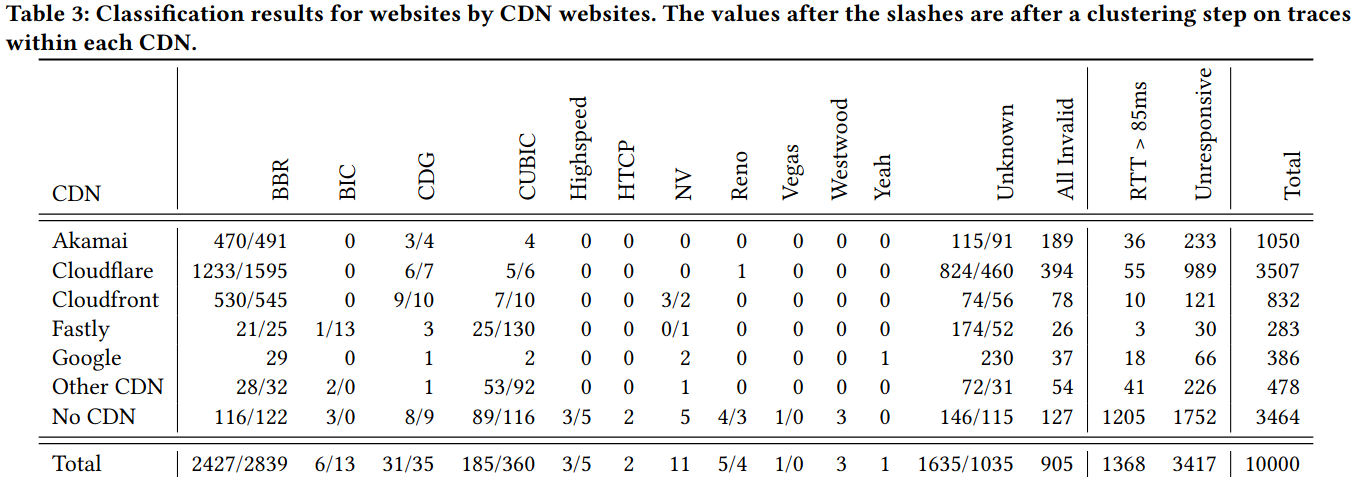
\includegraphics[width=\textwidth]{../congest/ware-et-al-table3}
\imagecredit{Ware et al, ``CCAnalyzer: An Efficient and Nearly Passive Congestion Control Classifier'}
\end{frame}

\begin{frame}
\frametitle{obtaining these measurements}
\begin{itemize}
\item Ware et al (2024) technique: estimate queue occupancy
    \begin{itemize}
    \item add artificial slow link on measurement path
    \item measure number of packets queued over time
    \item shape of graph indicates which congestion control algorithm
    \end{itemize}
\end{itemize}
    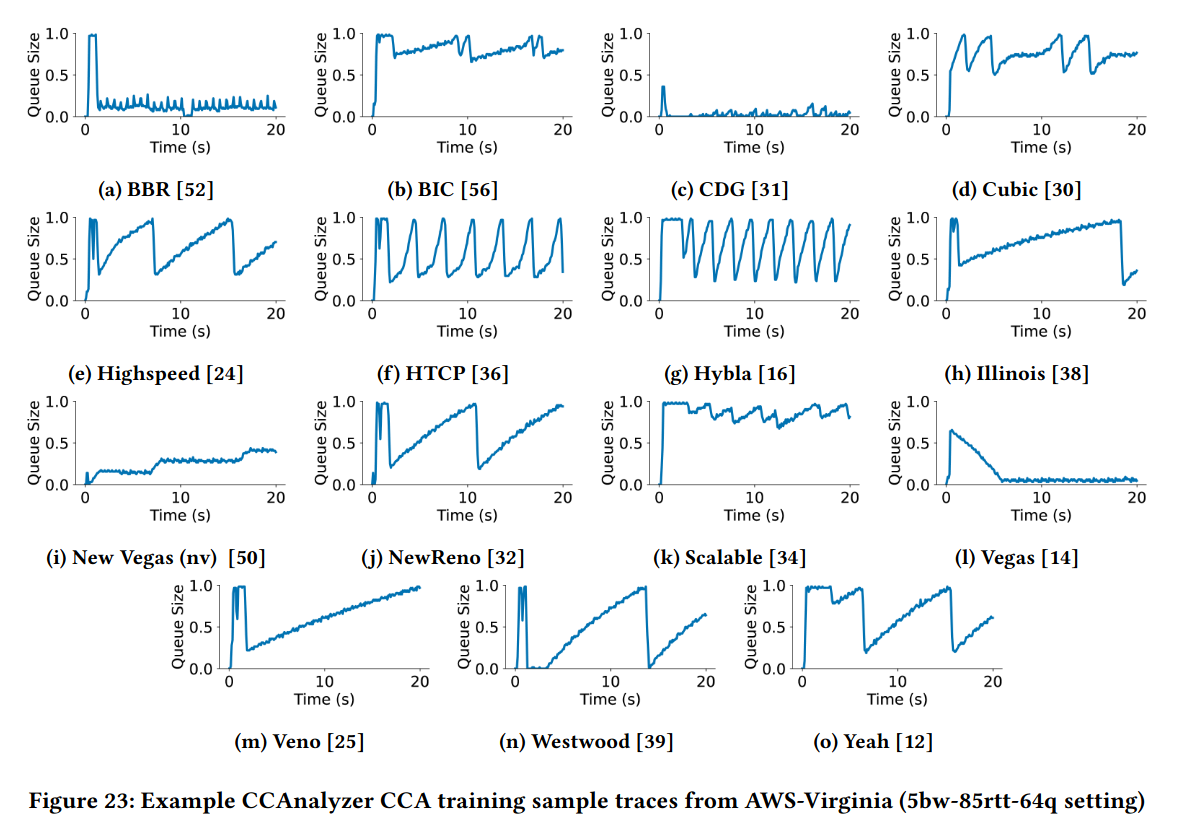
\includegraphics[height=0.5\textheight]{../congest/ware-et-al-fig23}
\end{frame}
